\documentclass[11pt,a4paper]{article}
\usepackage[T1]{fontenc}
\usepackage{lmodern}
\usepackage[margin=2.2cm]{geometry}
\usepackage{amsmath,amssymb}
\usepackage{booktabs,tabularx,array}
\usepackage{graphicx}
\usepackage{float}
\usepackage{longtable}
\usepackage{xcolor}
\usepackage{tikz}
\usetikzlibrary{arrows.meta,positioning}
\usepackage[hidelinks]{hyperref}
\def\sectionautorefname{Section}\def\subsectionautorefname{Section}

\definecolor{navy}{HTML}{1F3A5F}
\definecolor{soft}{HTML}{EEF3FA}
\definecolor{todo}{HTML}{FDF1E9}
\definecolor{todoline}{HTML}{EB6834}
\newcommand{\code}[1]{\texttt{\small #1}}
% A box the author fills in: the course does not allow LLM-written analysis or conclusions.
\newcommand{\authorbox}[2]{\par\smallskip\noindent\fcolorbox{todoline}{todo}{\parbox{\dimexpr\linewidth-2\fboxsep-2\fboxrule}{%
  \small\textbf{To be written by the author --- #1}\par\smallskip #2}}\par\smallskip}

% generated by make_figures.py
\newcommand{\argmaxEtwo}{0.3730}
\newcommand{\bestconf}{0.518}
\newcommand{\bestconfname}{E2 (A4 LoRMA, original backbone), prop10}
\newcommand{\bestconfsd}{0.016}
\newcommand{\confEtwocleanBnone}{0.467}
\newcommand{\confEtwocleanBnonesd}{0.010}
\newcommand{\confEtwocleanBprop}{0.479}
\newcommand{\confEtwocleannone}{0.479}
\newcommand{\confEtwocleannonesd}{0.013}
\newcommand{\confEtwocleanprop}{0.496}
\newcommand{\confEtwonone}{0.488}
\newcommand{\confEtwononesd}{0.007}
\newcommand{\confEtwoprop}{0.518}
\newcommand{\efEfive}{0.4697}
\newcommand{\efEfour}{0.3892}
\newcommand{\efEone}{0.4267}
\newcommand{\efEsix}{0.3443}
\newcommand{\efEthree}{0.3564}
\newcommand{\efEtwo}{0.4857}
\newcommand{\errboundary}{8.0}
\newcommand{\errboundlabel}{2.9}
\newcommand{\errexact}{45.7}
\newcommand{\errmissed}{37.9}
\newcommand{\errspurious}{195}
\newcommand{\errwronglabel}{5.6}
\newcommand{\kdparams}{52.9M}
\newcommand{\lconefive}{0.339}
\newcommand{\lcsixzero}{0.486}
\newcommand{\lcthreezero}{0.448}
\newcommand{\maxwords}{19,978}
\newcommand{\medwords}{4,488}
\newcommand{\nsweep}{37}
\newcommand{\ntestdocs}{35}
\newcommand{\ntraindocs}{70}
\newcommand{\oraclenosplit}{0.9866}
\newcommand{\oraclesplit}{0.9945}
\newcommand{\propfiveEtwo}{0.5142}
\newcommand{\teacherparams}{81.3M}
\newcommand{\topconfusions}{APP$\to$RESP 35, PREC$\to$APP 11, PREC$\to$RESP 10, WIT$\to$PREC 9, WIT$\to$RESP 7, APP$\to$PREC 7, APP$\to$AUTH 7, PREC$\to$JUDGE 7}
\newcommand{\totents}{8,393}
\newcommand{\viterbiEtwo}{0.4857}

\makeatletter\newcommand{\tabinput}[1]{\@@input #1 }\makeatother % expandable \input inside tabulars

\title{\textbf{CS-781 Capstone, Phase 2: Legal Named Entity Recognition}\\[2pt]
\large Character-level legal NER on the four Phase-1 language models}
\author{Manish Kumar (251330604)\\ CS-781, IIT Kanpur}
\date{October 2026}

\begin{document}
\maketitle

\begin{abstract}
\noindent We tag twelve legal entity types (parties, counsel, judges, witnesses, authorities, courts,
statutes, precedents, dates and case numbers) as character spans in long Indian judgments, starting from the
four language models we pre-trained in Phase~1.  A shared pipeline converts character spans to BIO token tags
and back (oracle macro-F1 \oraclesplit{} with punctuation pre-splitting), runs each backbone as a token
encoder, and decodes with a BIO-constrained Viterbi.  Six submissions cover all four architectures and five
adaptation methods: full fine-tuning (A3), LoRMA+ (A4), LoRA (A1), Houlsby adapters (A2), partial
fine-tuning (A4) and knowledge distillation into a 4-block A3 student.  A4 with LoRMA+ scores the highest
dev strict macro-F1 (\efEtwo).  A sweep of \nsweep{} one-change variants, an inference-only decoding sweep
and a three-split confirmation follow; the best confirmed setting is \bestconfname{}
(\bestconf$\pm$\bestconfsd).  An error analysis shows that \errmissed\% of gold entities are not predicted
at all.  All numbers are generated from the run outputs by \code{p2/report/make\_figures.py}.
\end{abstract}

\tableofcontents
\newpage

% =====================================================================
\section{Introduction}
Legal named entity recognition (L-NER) identifies entities by their \emph{legal role}: not just a person,
but the appellant, the respondent, their counsel, a witness or the judge.  Phase~2 asks for the character
start and end offset and the label of every entity in a judgment; scoring is strict (span and label must
both match exactly) and the primary metric is macro-F1 over the twelve labels.  The rules require the
Phase-1 models as the only pretrained weights, all four Phase-1 architectures across the submissions, at
least five different fine-tuning or parameter-efficient techniques, and knowledge distillation; at least six
submissions are needed.

The report follows the work in order: the data (\autoref{sec:data}), the character/token pipeline
(\autoref{sec:pipeline}), the backbones and adaptation methods (\autoref{sec:methods}), the six experiments
(\autoref{sec:res-main}), the tuning sweep, decoding sweep and three-split confirmation
(\autoref{sec:res-sweep} to \autoref{sec:res-confirm}), the learning curve (\autoref{sec:res-lc}), an error
analysis (\autoref{sec:res-err}) and the effect of the cleaned Phase-1 backbones (\autoref{sec:res-clean}).

% =====================================================================
\section{Data}\label{sec:data}
\begin{itemize}
  \item \textbf{Training}: \ntraindocs{} documents (two folds of 35) with gold spans as
  \code{[start, end, label, text]}; \textbf{test}: \ntestdocs{} documents without labels.
  \item Documents are long: median \medwords{} words, maximum \maxwords{} words, against a 1{,}024-token
  Phase-1 context.
  \item \totents{} gold entities over twelve labels (\autoref{tab:labels}); counsel, judges and witnesses have
  fewer than 250 examples each.
  \item \textbf{Dev split}: 10 of the 70 documents (\code{data.split\_seed}=0) are held out for model
  selection and every comparison, the same for every run.  For the confirmation (\autoref{sec:res-confirm})
  two more disjoint-ish splits (seeds 1, 2) are used.
\end{itemize}

\begin{table}[H]\centering\small
\caption{Gold entities per label in the 70 training documents.}\label{tab:labels}
\begin{tabular}{lr}\toprule Label & Entities\\\midrule
\tabinput{tables/labels.tex}
\bottomrule\end{tabular}\end{table}

% =====================================================================
\section{From characters to tags and back}\label{sec:pipeline}
\begin{figure}[H]\centering
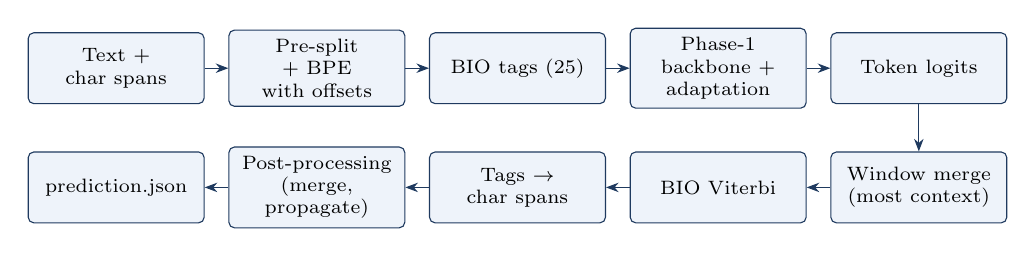
\begin{tikzpicture}[node distance=3mm, box/.style={draw=navy,rounded corners=2pt,fill=soft,align=center,
  font=\scriptsize,minimum height=9mm,text width=20mm}, arr/.style={-{Stealth[length=1.6mm]},navy}]
  \node[box] (a) {Text + char spans};
  \node[box,right=of a] (b) {Pre-split + BPE with offsets};
  \node[box,right=of b] (c) {BIO tags (25)};
  \node[box,right=of c] (d) {Phase-1 backbone + adaptation};
  \node[box,right=of d] (e) {Token logits};
  \node[box,below=6mm of e] (f) {Window merge (most context)};
  \node[box,left=of f] (g) {BIO Viterbi};
  \node[box,left=of g] (h) {Tags $\to$ char spans};
  \node[box,left=of h] (i) {Post-processing (merge, propagate)};
  \node[box,left=of i] (j) {prediction.json};
  \foreach \x/\y in {a/b,b/c,c/d,d/e,e/f,f/g,g/h,h/i,i/j} \draw[arr] (\x)--(\y);
\end{tikzpicture}
\caption{The L-NER pipeline (\code{lner/data.py}, \code{lner/engine.py}, \code{lner/decoding.py}).}
\label{fig:pipeline}\end{figure}

\begin{itemize}
  \item \textbf{Tokenisation with offsets.} The Phase-1 byte-level BPE (32k) encodes the text and returns the
  character offsets of every token, with the leading space of a token excluded.
  \item \textbf{Punctuation pre-splitting} (\code{data.presplit}). Legal text has runs such as \code{).} and
  \code{],}; an entity often ends in the middle of one, so BPE merges the entity's last character with the
  following punctuation.  Cutting punctuation runs into separate pieces before BPE puts more entity
  boundaries on token boundaries.
  \item \textbf{BIO tags.} A token that overlaps a gold span gets \code{B-}/\code{I-}\textit{label}, the rest
  \code{O}: 25 tags.
  \item \textbf{Oracle check} (\code{scripts/check\_alignment.py}). Encoding the gold spans as tags and decoding
  them back gives the best score any tagger can reach with this tokenisation: macro-F1 \oraclenosplit{}
  without pre-splitting and \oraclesplit{} with it.
  \item \textbf{Windows.} Training uses 512-token windows with stride 256 and a random shift each epoch.
  Inference uses stride 128; each token keeps the logits of the window in which it has the most context on
  both sides.
  \item \textbf{Decoding.} Viterbi over the tag logits with transitions that break BIO (e.g.\ \code{O}$\to$
  \code{I-X}) forbidden; \code{argmax} is the unconstrained alternative.  Tags are mapped back to character
  spans with trailing whitespace trimmed.
  \item \textbf{Post-processing} (inference only, \autoref{sec:res-dec}). \emph{merge}: two consecutive spans
  with the same label separated only by spaces are joined.  \emph{propagate}$k$: a string predicted as an
  entity (at least $k$ characters) is also tagged, with its majority label, wherever else it appears as a
  whole word untagged in the same document.
  \item \textbf{Metrics} (\code{lner/metrics.py}). Strict macro precision/recall/F1 as on Codabench, plus
  micro-F1 and \emph{span-only} F1 (boundaries right, label ignored) for error analysis.
\end{itemize}

% =====================================================================
\section{Methods}\label{sec:methods}
\subsection{Backbones}
The Phase-1 model returns one hidden vector per token (\code{lner/backbones.py}); the language-model head
is replaced by a token-classification head (linear by default; an MLP and a CRF head \cite{lafferty2001crf} were also tried).
\begin{itemize}
  \item \textbf{A1 GPT} and \textbf{A4 efficient}: either the Phase-1 causal mask is kept
  (\code{attention: causal}, a token sees only its left context) or removed (\code{bidirectional}; A4's local
  layers then see $\pm$256 tokens).  The six experiments use bidirectional attention.
  \item \textbf{A3 prefix-LM}: the whole window is treated as the bidirectional prefix.
  \item \textbf{A2 encoder--decoder}: either the encoder output alone, or the decoder run over the same window
  while cross-attending to the encoder (\code{encdec\_output: decoder}, BART-style tagging).
\end{itemize}

\paragraph{A2 diagnostic.} Tagging from the A2 encoder output gave dev macro-F1 of only 0.11--0.15
(\autoref{tab:main}, ``enc.'' rows).  The mean cosine similarity between token vectors of the Phase-1 A2
encoder output is 0.92, against 0.19 for A3 (measured once, \code{p2/README.md}): the encoder output is
nearly collapsed and the decoder does most of the language modelling.  E4 therefore uses the decoder states.

\subsection{Adaptation methods}\label{sec:peft}
All implementations are in \code{lner/peft.py}, written from the papers; the head is always trained.
\begin{itemize}
  \item \textbf{Full fine-tuning}: every backbone weight.
  \item \textbf{Partial (layer-wise) fine-tuning}: only the top $n$ blocks and the final norm (E5: top 4 of 10).
  \item \textbf{LoRA} \cite{hu2022lora}: a frozen linear layer $W_0$ gets an additive low-rank update,
  $h = W_0x + \frac{\alpha}{r}BAx$ with $B=0$ at initialisation.
  \item \textbf{LoRMA+} \cite{bihany2025lorma}: a multiplicative low-rank update,
  $W = (I + \frac{\alpha}{r}BA)\,W_0$, computed as $h_0=W_0x$, $h = h_0 + \frac{\alpha}{r}B(Ah_0)$ so its cost
  matches LoRA.  \textbf{LoRMA$_\pi$} (sweep only) replaces $I + BA$ by a rank-inflating permutation of $BA$
  initialised to the identity.
  \item \textbf{Houlsby adapters} \cite{houlsby2019adapters}: a bottleneck MLP ($d\to64\to d$, up-projection
  initialised to zero) after the attention and the MLP sub-layers; layer norms are also trained.
  \item \textbf{BitFit} \cite{benzaken2022bitfit} (sweep): only biases and norm gains.
  \item \textbf{IA$^3$} \cite{liu2022ia3} (sweep): learned scaling of keys, values and the MLP's inner
  activation, initialised to one.
  \item \textbf{Knowledge distillation} \cite{hinton2015kd} (E6): the student is A3 with 4 of its 8 blocks
  (blocks 1, 3, 5, 7; \kdparams{} parameters against \teacherparams{} for the teacher), fully fine-tuned with
  $\mathcal{L} = \alpha\,\mathrm{CE} + (1-\alpha)\,T^2\,\mathrm{KL}(p_\text{teacher}^{T} \,\|\, p_\text{student}^{T})$,
  $\alpha=0.5$, $T=2$, teacher E1 (A3 full fine-tuning).
\end{itemize}
LoRA-family methods wrap the attention projections (\code{q k v o}) and the MLP projections, with $r=16$,
$\alpha=32$, dropout 0.05.

\subsection{Training}
AdamW, 15 epochs with early stopping after 5 epochs without dev improvement (best epoch kept), batch 16
windows, 10\% linear warm-up then cosine decay, weight decay 0.01, gradient clipping 1.0.  Learning rate
$10^{-3}$ for LoRA/LoRMA/adapters, $2\times10^{-4}$ for partial and KD, $10^{-4}$ for full fine-tuning; the
head always uses $10^{-3}$.  The loss is token cross-entropy; the sweep also tries an \code{O}-tag weight,
inverse-square-root class weights, focal loss \cite{lin2017focal}, layer-wise LR decay, dropout and a CRF head.
Only trainable parameters are saved, so PEFT checkpoints are a few MB.

\subsection{The six experiments}
\begin{table}[H]\centering\small
\caption{Submitted experiments (\code{p2/configs/}).}\label{tab:exps}
\begin{tabular}{lllll}\toprule
ID & Phase-1 model & Method & Config & Notes\\\midrule
E1 & A3 prefix-LM & full fine-tuning & \code{e1\_a3\_full.yaml} & KD teacher\\
E2 & A4 efficient & LoRMA+ & \code{e2\_a4\_lorma.yaml} & mandatory LoRMA\\
E3 & A1 GPT & LoRA & \code{e3\_a1\_lora.yaml} & \\
E4 & A2 enc--dec & Houlsby adapters & \code{e4\_a2\_adapter.yaml} & decoder states\\
E5 & A4 efficient & partial (top 4 blocks) & \code{e5\_a4\_partial.yaml} & \\
E6 & A3, 4 of 8 blocks & KD from E1 & \code{e6\_kd\_a3\_small.yaml} & mandatory KD\\
\bottomrule\end{tabular}\end{table}

% =====================================================================
\section{Results}
\subsection{The six experiments}\label{sec:res-main}
\begin{table}[H]\centering\scriptsize\setlength{\tabcolsep}{3.5pt}
\caption{Dev split 0 (10 documents). Span = span-only F1. Time in minutes; memory = peak GPU allocation.}
\label{tab:main}
\resizebox{\linewidth}{!}{\begin{tabular}{lllrrrrrrrrrr}\toprule
Run & Arch & Method & Trainable & \% & Macro-F1 & P & R & Micro-F1 & Span & Min & GB & MB\\\midrule
\tabinput{tables/main.tex}
\bottomrule\end{tabular}}\end{table}

\begin{figure}[H]\centering
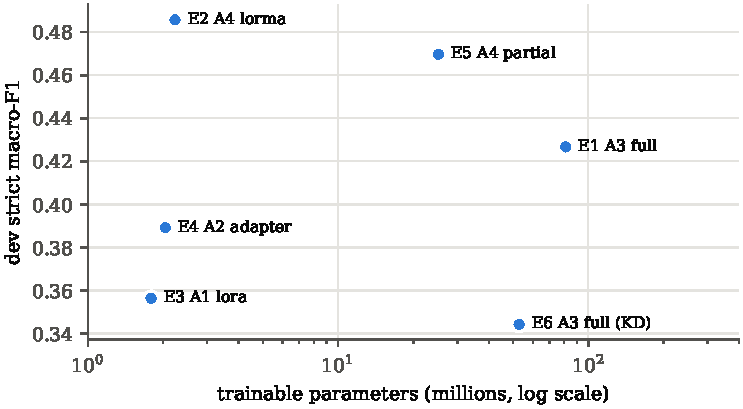
\includegraphics[width=0.78\linewidth]{figs/f1_vs_params.pdf}
\caption{Dev macro-F1 against the number of trained parameters.}
\label{fig:params}\end{figure}

\begin{figure}[H]\centering
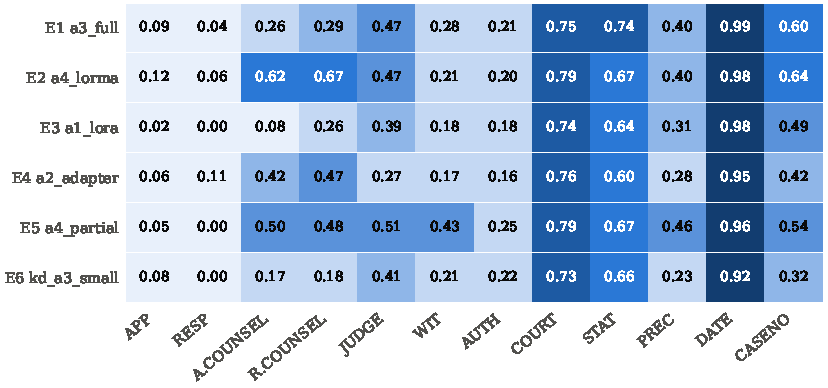
\includegraphics[width=0.95\linewidth]{figs/per_label.pdf}
\caption{Dev F1 per label for the six experiments.}
\label{fig:perlabel}\end{figure}

\subsection{One-change sweep}\label{sec:res-sweep}
Each variant changes one thing in one of the experiments (the ``change'' column is the difference between
the two \code{config.yaml} files).  All are scored on dev split 0, so a single difference of about $\pm$0.02
is within the split-to-split variation measured in \autoref{sec:res-confirm}.

\begin{figure}[H]\centering
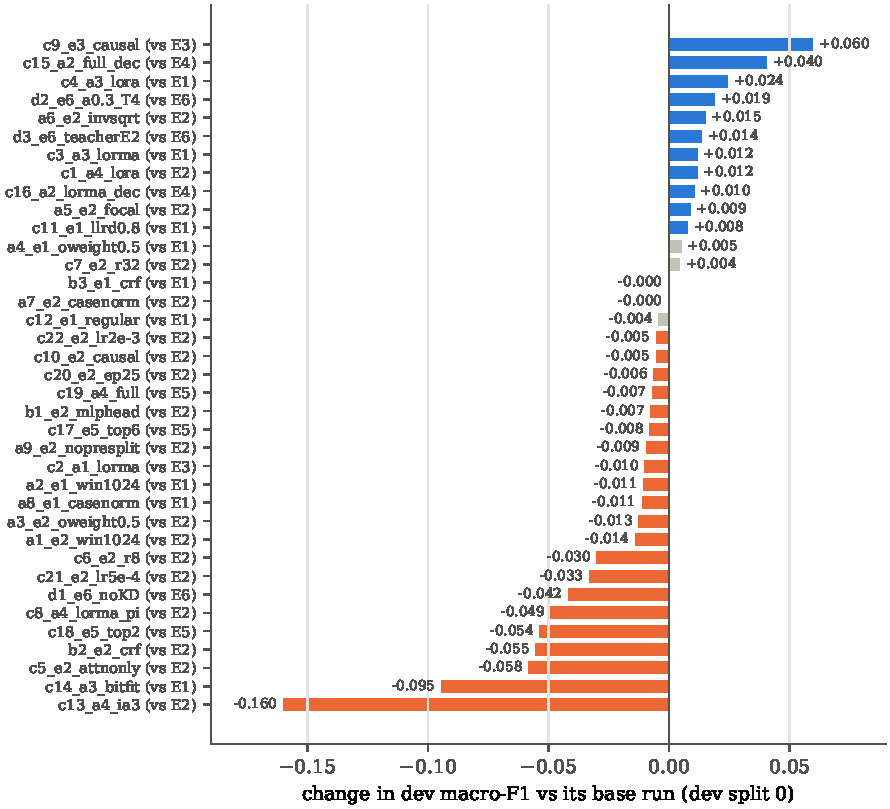
\includegraphics[width=0.85\linewidth]{figs/sweep_deltas.pdf}
\caption{Change in dev macro-F1 of each variant against its base experiment (blue: $>$+0.005, orange:
$<-$0.005, grey: in between).}
\label{fig:sweep}\end{figure}

{\scriptsize\setlength{\tabcolsep}{3pt}
\begin{longtable}{llp{6.3cm}rrrr}\caption{One-change sweep (\code{sweeps/RESULTS.md}).}\label{tab:sweep}\\\toprule
Variant & Base & Change & Base F1 & F1 & $\Delta$ & Span\\\midrule\endfirsthead
\toprule Variant & Base & Change & Base F1 & F1 & $\Delta$ & Span\\\midrule\endhead
\tabinput{tables/sweep.tex}
\bottomrule\end{longtable}}

\subsection{Decoding and post-processing}\label{sec:res-dec}
The trained E1, E2 and E5 models are re-decoded with different inference strides, decoders and
post-processing, without retraining (\code{scripts/infer\_sweep.py}).  For E2 at stride 128: argmax
\argmaxEtwo{}, BIO Viterbi \viterbiEtwo{}, Viterbi + propagate5 \propfiveEtwo{}.

\begin{figure}[H]\centering
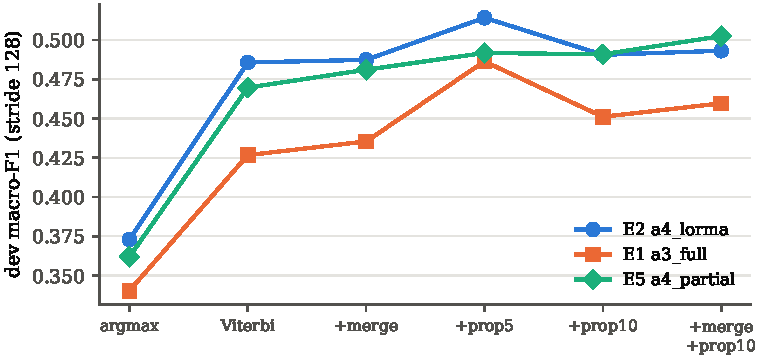
\includegraphics[width=0.78\linewidth]{figs/decoding.pdf}
\caption{Dev macro-F1 for each decoding / post-processing option (stride 128).}
\label{fig:decoding}\end{figure}

\begin{table}[H]\centering\scriptsize
\caption{Inference-only sweep: macro-F1 at strides 64 / 128 / 256, and precision / recall at stride 128.}\label{tab:inference}
\begin{tabular}{llrrrrr}\toprule
Run & Decoding & 64 & 128 & 256 & P & R\\\midrule
\tabinput{tables/inference.tex}
\bottomrule\end{tabular}\end{table}

\subsection{Three-split confirmation}\label{sec:res-confirm}
The most promising settings were retrained on dev splits 0, 1 and 2 (\code{scripts/confirm.py}) and scored
with every post-processing option.

\begin{figure}[H]\centering
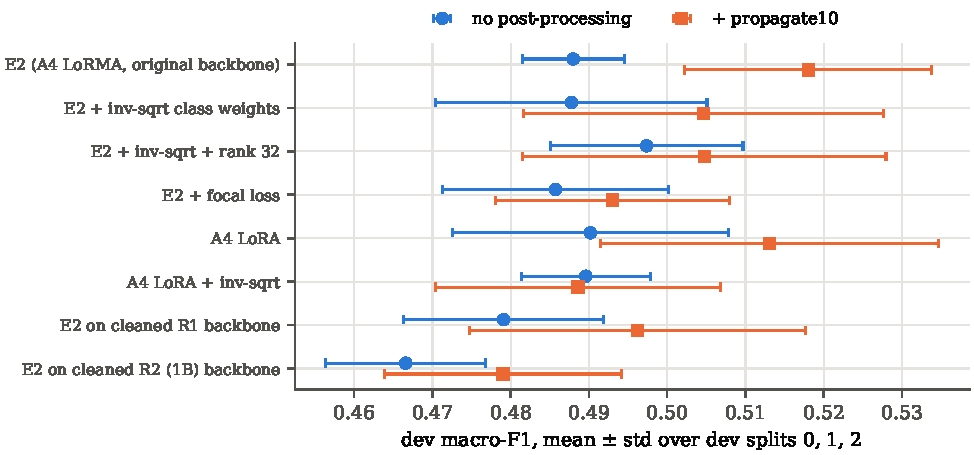
\includegraphics[width=0.88\linewidth]{figs/confirm.pdf}
\caption{Mean $\pm$ standard deviation over three dev splits, without post-processing and with
propagate10.}
\label{fig:confirm}\end{figure}

\begin{table}[H]\centering\scriptsize\setlength{\tabcolsep}{3pt}
\caption{Dev macro-F1, mean $\pm$ std over three dev splits, per post-processing option.}\label{tab:confirm}
\begin{tabular}{lrrrrrr}\toprule
Setting & none & merge & prop5 & prop10 & merge+prop5 & merge+prop10\\\midrule
\tabinput{tables/confirm.tex}
\bottomrule\end{tabular}\end{table}

\subsection{Learning curve}\label{sec:res-lc}
E2 retrained on 15 and 30 of the 60 training documents of split 0 (\code{data.max\_train\_docs}):
\lconefive{}, \lcthreezero{} and \lcsixzero{} dev macro-F1 for 15, 30 and 60 documents.

\begin{figure}[H]\centering
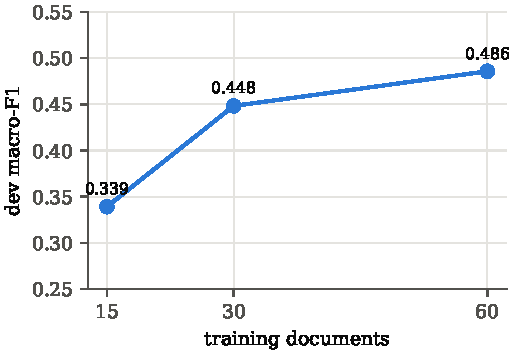
\includegraphics[width=0.48\linewidth]{figs/learning_curve.pdf}
\caption{E2 dev macro-F1 against the number of training documents.}
\label{fig:lc}\end{figure}

\subsection{Error analysis}\label{sec:res-err}
\code{scripts/error\_analysis.py} matches every gold entity of E2's dev predictions by overlap:
\emph{exact} (true positive), \emph{wrong label} (same span), \emph{boundary} (overlapping prediction with the
same label), \emph{boundary + label}, or \emph{missed} (no overlapping prediction).  Over all labels:
exact \errexact\%, wrong label \errwronglabel\%, boundary \errboundary\%, boundary + label \errboundlabel\%,
missed \errmissed\%; \errspurious{} predictions overlap no gold entity.  Most frequent confusions (gold
$\to$ predicted): \topconfusions.

\begin{figure}[H]\centering
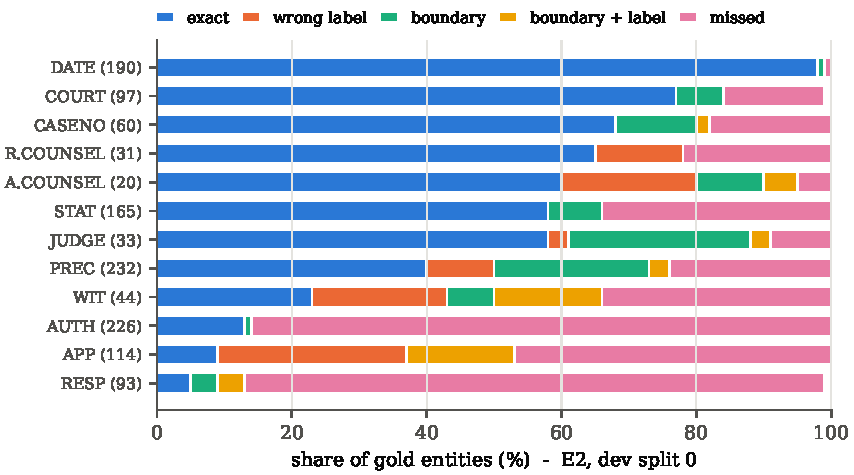
\includegraphics[width=0.88\linewidth]{figs/errors.pdf}
\caption{What happens to each gold entity of E2 on dev split 0, per label (gold count in brackets).}
\label{fig:errors}\end{figure}

\begin{table}[H]\centering\small
\caption{Error breakdown per label (E2, dev split 0); spurious = predictions overlapping no gold entity.}\label{tab:errors}
\begin{tabular}{lrrrrrrr}\toprule
Label & Gold & Exact & Wrong label & Boundary & Bound.+label & Missed & Spurious\\\midrule
\tabinput{tables/errors.tex}
\bottomrule\end{tabular}\end{table}

\subsection{Cleaned Phase-1 backbones}\label{sec:res-clean}
After Phase~1 was retrained on a cleaned corpus (Phase-1 report), the E2 recipe was rerun unchanged on the
new A4 checkpoints over the same three dev splits (\autoref{tab:confirm}, last two rows): original backbone
\confEtwonone$\pm$\confEtwononesd, cleaned R1 (200M tokens) \confEtwocleannone$\pm$\confEtwocleannonesd,
cleaned R2 (1B tokens) \confEtwocleanBnone$\pm$\confEtwocleanBnonesd{} without post-processing;
\confEtwoprop, \confEtwocleanprop{} and \confEtwocleanBprop{} with propagate10.  The submitted Phase-2
models use the original backbones.

\subsection{Submissions}
One Codabench zip per experiment, \code{prediction.json} at the root (\code{p2/submissions/}).
\authorbox{leaderboard scores}{Add the Codabench test macro-F1 of each submission here.}

% =====================================================================
\section{Analysis}
\authorbox{analysis of the results}{The course rules do not allow LLM-written result analysis.  Questions the
course asks (§8.7, §20.1), with the evidence above:
\begin{itemize}
  \item Which adaptation technique and which Phase-1 architecture work best for L-NER, and why
  (\autoref{tab:main}, \autoref{fig:params})?
  \item Can parameter-efficient methods approach full fine-tuning?
  \item Does distillation keep performance while reducing size?
  \item Which entity types are hard, and is the problem labels, boundaries or recall
  (\autoref{fig:perlabel}, \autoref{fig:errors})?
  \item What did the sweep teach, given the split-to-split variation (\autoref{fig:sweep},
  \autoref{fig:confirm})?
  \item Why might a better Phase-1 language model not give better NER (\autoref{sec:res-clean})?
  \item What failed, and why (A2 encoder, CRF head, IA$^3$, BitFit)?
\end{itemize}}

\section{Limitations and next steps}
Facts that limit the conclusions (the interpretation is the author's):
\begin{itemize}
  \item Model selection and every comparison use 10 dev documents; most sweep differences are within the
  split-to-split standard deviation (0.007--0.043 in \autoref{tab:confirm}).
  \item One seed per run.
  \item Windows of 512 tokens against documents of median \medwords{} words; party roles are stated in the
  header and must be resolved thousands of tokens later.
  \item 70 labelled documents; the learning curve (\autoref{fig:lc}) was still rising at 60.
  \item Post-processing is document-level but rule-based; it is not used during training.
\end{itemize}
\authorbox{what you would do next}{With more time or compute: \ldots}

\section{Conclusions}
\authorbox{conclusions}{Summarise what you conclude from the experiments, in your own words.}

\section{Reproducibility}
\noindent{\small\begin{tabularx}{\linewidth}{l>{\raggedright\arraybackslash}X}
All six experiments + zips & \code{bash run\_all.sh} (or \code{bash run\_all.sh e3})\\
One experiment & \code{python train.py --config configs/e2\_a4\_lorma.yaml}\\
Override a setting & \code{python train.py --config configs/e2\_a4\_lorma.yaml --set peft.r=8 run\_name=E2\_r8}\\
Predict / dev report & \code{python predict.py --run runs/E2\_a4\_lorma --split dev}\\
One-change sweep & \code{python scripts/sweep.py}\\
Decoding sweep & \code{python scripts/infer\_sweep.py}\\
Three-split confirmation & \code{python scripts/confirm.py}\\
Oracle alignment & \code{python scripts/check\_alignment.py}\\
Error analysis & \code{python scripts/error\_analysis.py runs/E2\_a4\_lorma}\\
Comparison table & \code{python scripts/compare.py}\\
Figures and tables & \code{python p2/report/make\_figures.py}\\
\end{tabularx}}
\authorbox{repository link}{GitHub: \url{https://github.com/...}}

\section*{LLM declaration}
\authorbox{LLM declaration (mandatory)}{Fill in the course questionnaire.  Describe honestly which parts used
an LLM assistant (for example the pipeline and PEFT code, sweep scripts, figures and this report's
methods/results text) and which parts are your own (design decisions, hyperparameters, analysis, conclusions).}

\begin{thebibliography}{99}\small
\bibitem{benzaken2022bitfit} E.~Ben Zaken, S.~Ravfogel, Y.~Goldberg. BitFit: Simple parameter-efficient fine-tuning for transformer-based masked language-models. ACL 2022.
\bibitem{bihany2025lorma} H.~Bihany, S.~Patel, A.~Modi. LoRMA: Low-rank multiplicative adaptation for LLMs. Findings of ACL 2025.
\bibitem{hinton2015kd} G.~Hinton, O.~Vinyals, J.~Dean. Distilling the knowledge in a neural network. arXiv:1503.02531, 2015.
\bibitem{houlsby2019adapters} N.~Houlsby et al. Parameter-efficient transfer learning for NLP. ICML 2019.
\bibitem{hu2022lora} E.~Hu et al. LoRA: Low-rank adaptation of large language models. ICLR 2022.
\bibitem{lafferty2001crf} J.~Lafferty, A.~McCallum, F.~Pereira. Conditional random fields. ICML 2001.
\bibitem{lin2017focal} T.-Y.~Lin et al. Focal loss for dense object detection. ICCV 2017.
\bibitem{liu2022ia3} H.~Liu et al. Few-shot parameter-efficient fine-tuning is better and cheaper than in-context learning. NeurIPS 2022.
\end{thebibliography}
\end{document}
